\chapter{Optimization with uncertain \texorpdfstring{$\alpha$}{alpha} functions}
\label{chap:unc_alpha}

\section{Contextual hypotesis}
\label{sec:unc_a_hyp}

We now assume that the binary features of the users cannot be observed and therefore data is considered as aggregated.

Since the features of the users are \textbf{not observable}, the $\alpha$ functions' shape for each class is unknown.

As a result, in our scenario the learner receives all the interactions minus the parameters of the $\alpha$ functions.

\section{Algorithm}
\label{sec:unc_a_alg}

By gathering the aggregated reward for each product we are able to utilize those coarse rewards to generate feedbacks for our MABs and therefore train them on the aggregated interactions for each day.

In particular, we exploit Gaussian Processes in conjunction with MAB algorithms such as Thompson Sampling and UCB1 to exploit the continuity between the different arms.
We instantiate a GP-MAB for each subcampaign and each MAB will have \texttt{n\_budget\_steps} number of arms.

\subsection{Algorithms outline}

The main two MAB algorithms that we are going to use present some minor variations when used in conjunction with Gaussian Processes; we can consider the GPTS algorithm as a baseline for the GPUCB1 since it directly uses the GPs' features to gather samples, while in the GPUCB1 we need to build a confidence bound before.

GPTS is a variant of TS implemented using Gaussian Processes that is implemented as follows:

\begin{itemize}
	\item For each day $t$, we gather a sample from each arm $a$:
		\begin{displaymath}
			\tilde{\theta_a} \leftarrow \text{ Sample} \left( \mathbb{P}(\mu_a = \theta_a) \right)
		\end{displaymath}
	\item Play arm $a_t$ defined as:
		\begin{displaymath}
			a_t \leftarrow arg\max_{a \in A} \left\{ \tilde{\theta_a} \right\}
		\end{displaymath}
	\item Update the Gaussian Process with the reward obtained.
\end{itemize}

Code snippets for updating the model and returning an estimation:

\begin{lstlisting}[style=Python]
def _update_model(self):
	x = np.atleast_2d(self.pulled_arms).T
	y = np.array(self.collected_rewards) / self.normalize_factor
	self.gp.fit(x, y)
	self.means, self.sigmas = self.gp.predict(
		np.atleast_2d(self.arms).T, return_std=True
	)
	self.sigmas = np.maximum(self.sigmas, 1e-2)
\end{lstlisting}

\begin{lstlisting}[style=Python]
def estimation(self):
	return self.rng.normal(
		self.means * self.normalize_factor, self.sigmas * self.normalize_factor
	)
\end{lstlisting}

GPUCB1 is a variant of UCB1 that takes advantage of the Gaussian Processes confidence interval and models it as the confidence bound; apart from the arm choice, the learning process is equal to GPTS. The arm choice is implemented as:

\begin{displaymath}
	a_t \leftarrow arg\max_{a \in A} \left\{ \mu_{t-1} + \delta \sigma_{t-1} \right\}
\end{displaymath}

Code snippet that calculates the upper bound:

\begin{lstlisting}[style=Python]
def estimation(self):
	upper_bounds = (self.means + self.confidence * 1.96 * self.sigmas)
			* self.normalize_factor
	return upper_bounds
\end{lstlisting}

\section{Results}
\label{sec:unc_a_res}

\subsection{Single run reward and regret}

Thompson Sampling and UCB

\begin{center}
	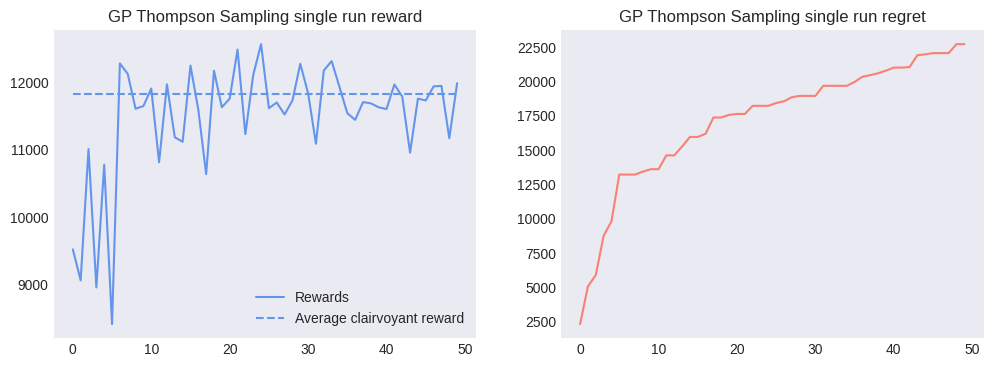
\includegraphics[scale=0.5]{img/Graphs/uncertain_alpha/image1.png}
	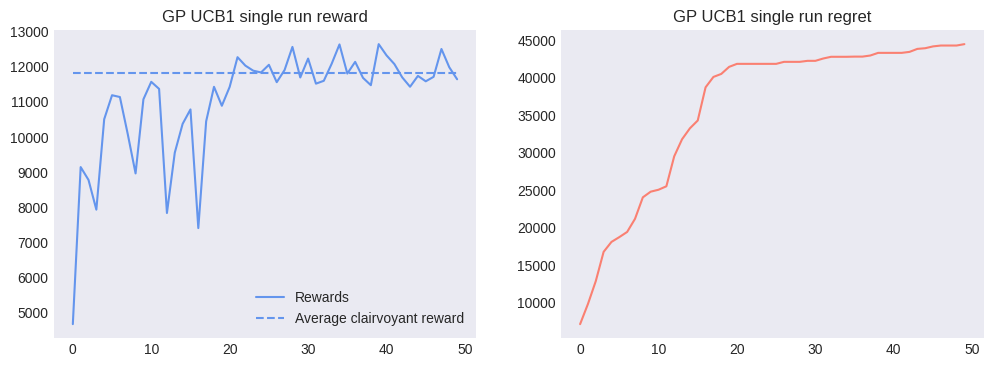
\includegraphics[scale=0.5]{img/Graphs/uncertain_alpha/image2.png}
\end{center}

Regret comparison

\begin{center}
	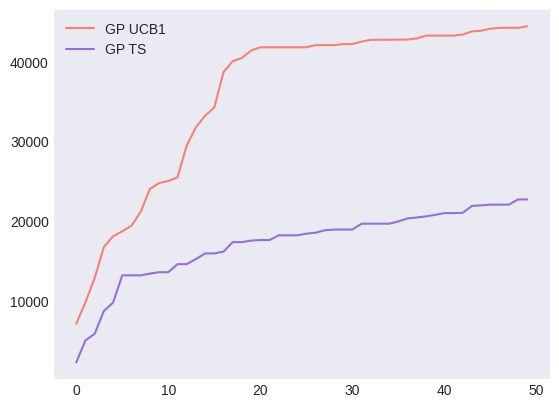
\includegraphics[scale=0.5]{img/Graphs/uncertain_alpha/image3.png}
\end{center}

\subsection{Average regret and reward}

Thompson Sampling and UCB

\begin{center}
	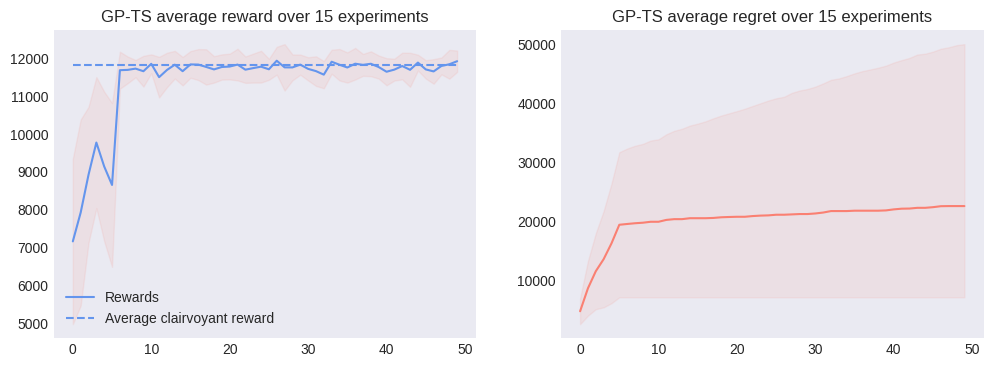
\includegraphics[scale=0.5]{img/Graphs/uncertain_alpha/image4.png}
	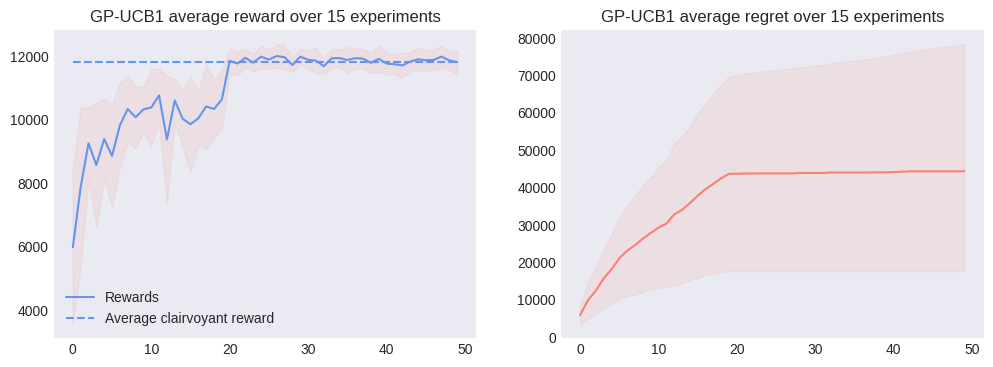
\includegraphics[scale=0.5]{img/Graphs/uncertain_alpha/image5.png}
\end{center}

Average regret comparison

\begin{center}
	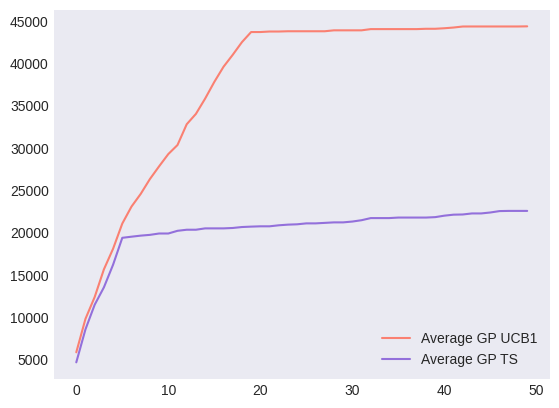
\includegraphics[scale=0.5]{img/Graphs/uncertain_alpha/image6.png}
\end{center}

\begin{displaymath}
	\text{Regret ratio } = \frac{\text{Avg regret}}{\text{Upper bound}} = \frac{31019.40}{?} = ?
\end{displaymath}

\todo{complete}

\subsection{Conclusions}

Overall we can observe more instability but a faster convergence in the TS algorithm w.r.t to the UCB approach.
However, both algorithms are able to converge to the optimal solution at different rates while respecting a linear cumulative regret bound.

Average results over 15 runs at time horizon $T = 50$:

\begin{table}[h]
	\center
	\begin{tabular}{|c|cc|c|}
	\hline \hline
		\cellcolor{blue!25} & Reward 	& Regret	& Deviation \\
	\cline{2-4}
		\cellcolor{blue!25} & $\mu$		& $\mu$		& $\sigma$	\\
	\hline \hline
		GPTS 				& 11610.53 	& 31024.67	& 440.36 	\\
	\hline
		GPUCB				& 11737.73	& 43686.67	& 349.47	\\
	\hline \hline
	\end{tabular}
\end{table}
